\documentclass{standalone}

\usepackage[latin1]{inputenc}
\usepackage{tikz}
\usepackage{amsmath}

\usetikzlibrary{calc}
\usetikzlibrary{arrows.meta}

\begin{document}

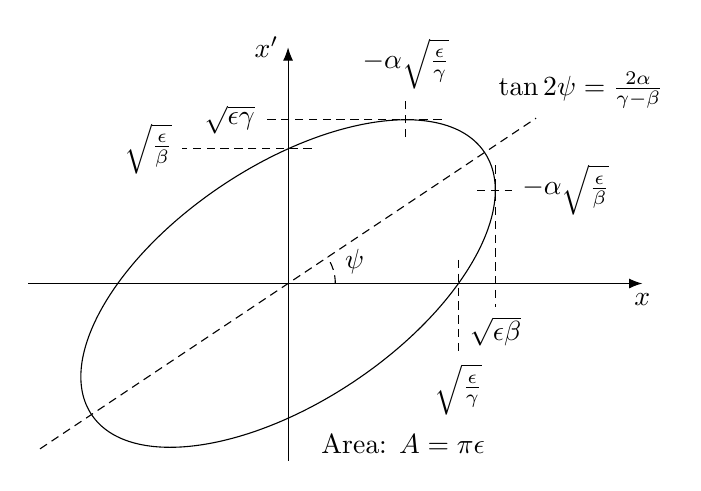
\begin{tikzpicture}[scale=3]
	% axes
	\draw[-Latex] (-1.1,0) -> (1.5,0) node[anchor=north] {\(x\)};
	\draw[-Latex] (0,-0.75) -> (0,1) node[anchor=east] {\(x'\)};

	% diagonal line
	\draw[densely dashed] (-1.5*0.7,-1*0.7) -- (1.5*0.7,1*0.7)
	node[anchor=south west, xshift=-0.6cm] {\(\tan2\psi = \frac{2\alpha}{\gamma-\beta}\)};
	
	% angle annotation
	\draw[densely dashed] (0.2,0) node[anchor=south west] {\(\psi\)} arc (0:33.6901:0.2);

	% ellipse
	\draw[rotate=33.6901] (0,0) ellipse (1 and 0.5);

	% x annotations
	\draw[densely dashed] (0.499, 0.62) -- (0.499, 0.78) node[anchor=south] {\(-\alpha\sqrt{\frac{\epsilon}{\gamma}}\)};
	\draw[densely dashed] (0.721, 0.1) -- (0.721, -0.3) node[anchor=north] {\(\sqrt{\frac{\epsilon}{\gamma}}\)};
	\draw[densely dashed] (0.878, 0.5) -- (0.878, -0.1) node[anchor=north] {\(\sqrt{\epsilon\beta}\)};

	% y annotations
	\draw[densely dashed] (0.8, 0.395) -- (0.95, 0.395) node[anchor=west] {\(-\alpha\sqrt{\frac{\epsilon}{\beta}}\)};
	\draw[densely dashed] (0.1, 0.570) -- (-0.45, 0.570) node[anchor=east] {\(\sqrt{\frac{\epsilon}{\beta}}\)};
	\draw[densely dashed] (0.65, 0.693) -- (-0.1, 0.693) node[anchor=east] {\(\sqrt{\epsilon\gamma}\)};

	\draw (0.1, -0.6) node[anchor=north west] {Area: \(A = \pi\epsilon\)};

\end{tikzpicture}

\end{document}
